\section{Structuration et programmation}

Quand j'étais arrivée, la structure de codes et celle de \db\ étaient définies par Ophir. Au début, j'ai continué avec celles d'Ophir, mais après le dégagement développement, les structures étaient changés. Dans ce chapitre, je vais montrer les changements structurels de \db\ et de codes, aussi des réalisations codage de certains parties de la plate-forme.

\subsection{Structuration de \db\ }

La \db\ était structurée selon la conception qui demande à garder tous les livres et layers dedans :

\begin{figure}[H]
\centering
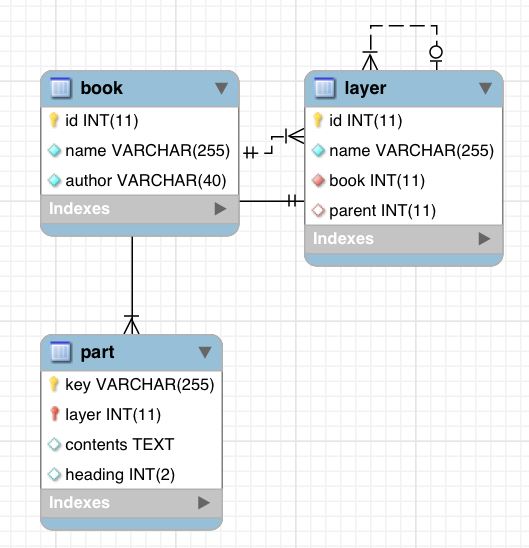
\includegraphics[width=\textwidth]{ancienne_structure}
\caption{L'ancienne structure de \db\ }
\end{figure}

Avec la conception d'utilisation d'XML, on va garder tous les livres et layers dans des fichiers XML. Pour l'instant, la norme utilisée par la plate-forme n'est pas encores définie, donc j'ai structuré un système permettant tous garder dans la \db\ . D'ailleurs, pour accéler des éditions, ça peut-être intéressant d'utiliser \db\ comme des caches entre des pages HTML et des XML. Pour cette question, je vais regarder DHWriter, un outil d'édition de open source ressenblant le GoogleDoc. 

Pour la parite de la gestion d'utilisateurs , la solution idéale est d'utiliser les systèmes d'accès des écoles, mais il faut aussi permet de s'inscire et manager le profil sur la plate-forme. Toutes informations de la gestion de groupes sont aussi gardés dans la \db\ :

\begin{figure}[H]
\centering
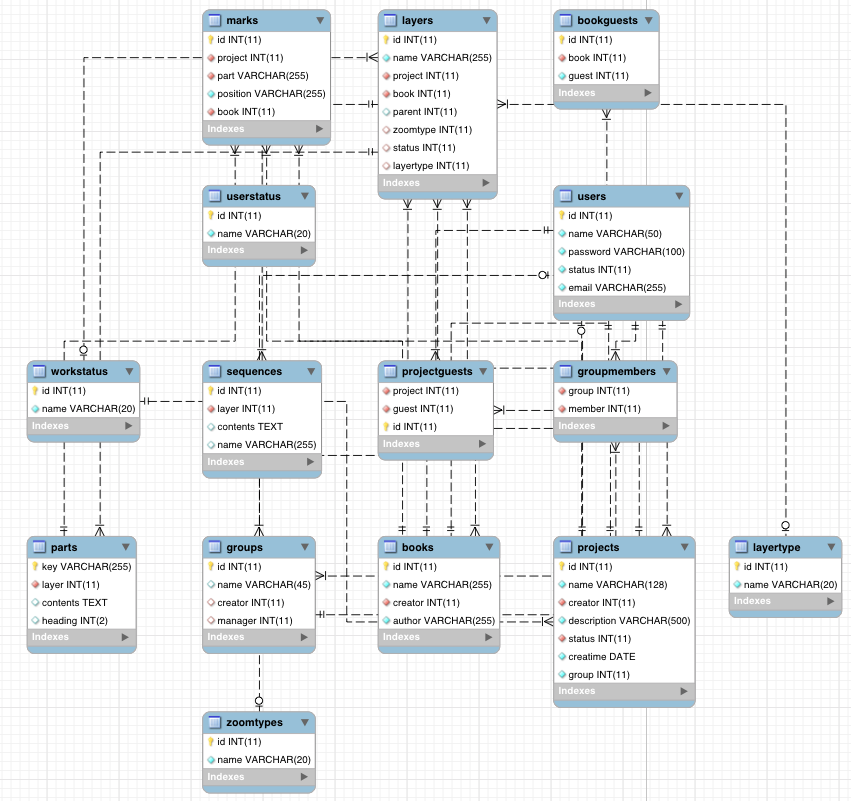
\includegraphics[width=\textwidth]{nouvelle_structure}
\caption{La nouvelle structure de \db\ }
\end{figure}

\subsection{Structuration de codes}

La structure de codes étaient aussi changé une fois avec l'avance de codes :

\begin{figure}[H] 
\begin{subfigure}{0.5\textwidth}
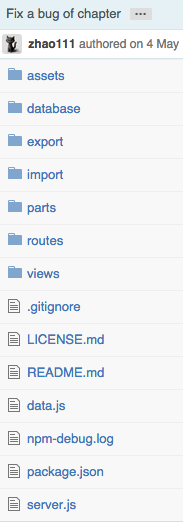
\includegraphics[width=0.7\linewidth]{ancienne_codes} 
\caption{L'ancienne structure de codes}
\label{fig:subim1}
\end{subfigure}
\begin{subfigure}{0.5\textwidth}
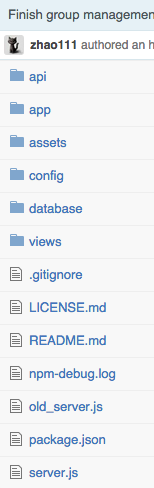
\includegraphics[width=0.62\linewidth]{codes}
\caption{La nouvelle structure de codes}
\label{fig:subim2}
\end{subfigure} 
\caption{Changements de la structure de codes}
\label{fig:image2}
\end{figure}

Dans la structure, le dossier \textbf{views} garde des fichiers .jsx controllents des pages de clients, le dossier \textbf{database} a des fichies .js chargeant des mises à jour de la \db\ , le dossier \textbf{assets} a des fichiers publiques, tous les modules utilisés sont configurés dans le fichier package.json et le server.js est l'entrée de codes défini la configuration des dossiers et des fichiers.

Les changements et raisons :

\begin{itemize}
    \item Supprimer le dossier \textbf{parts} utilisé plus avec l'idée d'XML
    \item Intégrer des fichiers dans le dossier \textbf{app} qui  et \textbf{api}
    \item Configurer des informations de la \db\ et d'autres modules dans le dossier \textbf{config}
\end{itemize}


\subsection{Réalisation de l'édition de transcription}

La première partie de codes j'ai réalisé est l'édition de transcription de l'ancienne conception. La réalisation  Les fonctions principales sont :

\begin{itemize}
    \item Créer un sous-layer en héritant des parties correspondantes à chaque paragraphe
    \item Cliquer sur le boutton Entre pour ajouter une partie avant la partie prochaine déjà avec des contenus
    \item Supprimer la partie quand on clique sur le boutton Delete dans une partie vide
    \item Mise à jours la \db\ avec tous les changement d'éditions quand on clique Save
\end{itemize}

En bref, la réalisation du page d'édition étais une imitation d'éditions habituelles qui a essayé de cacher la création, le transformation et la suppression de parties. 

\begin{figure}[H]
\centering
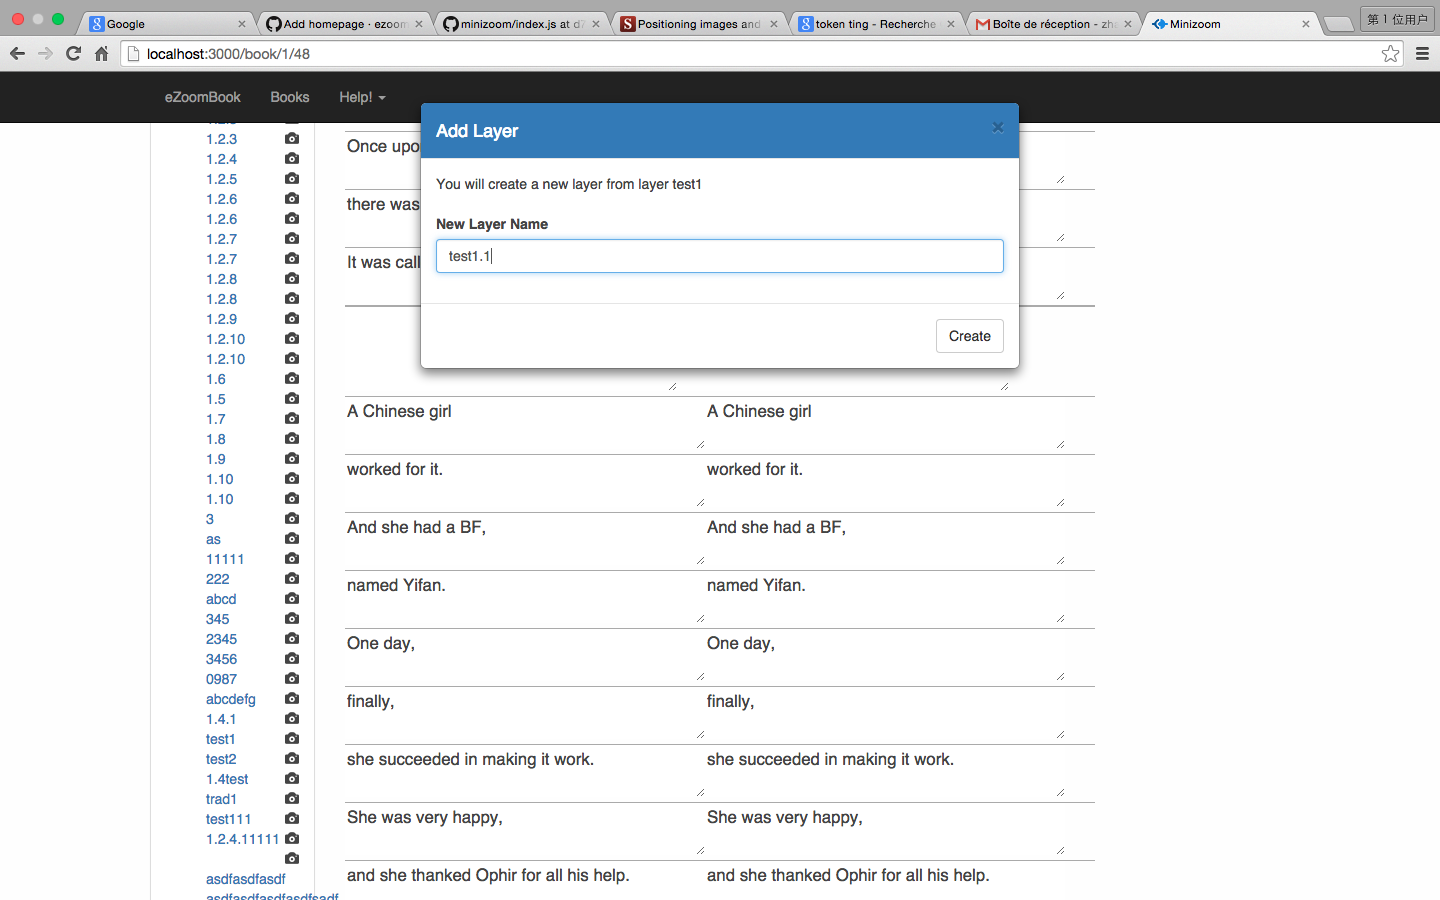
\includegraphics[width=\textwidth]{trans1}
\caption{Créer un nouveau layer}
\end{figure}

\begin{figure}[H]
\centering
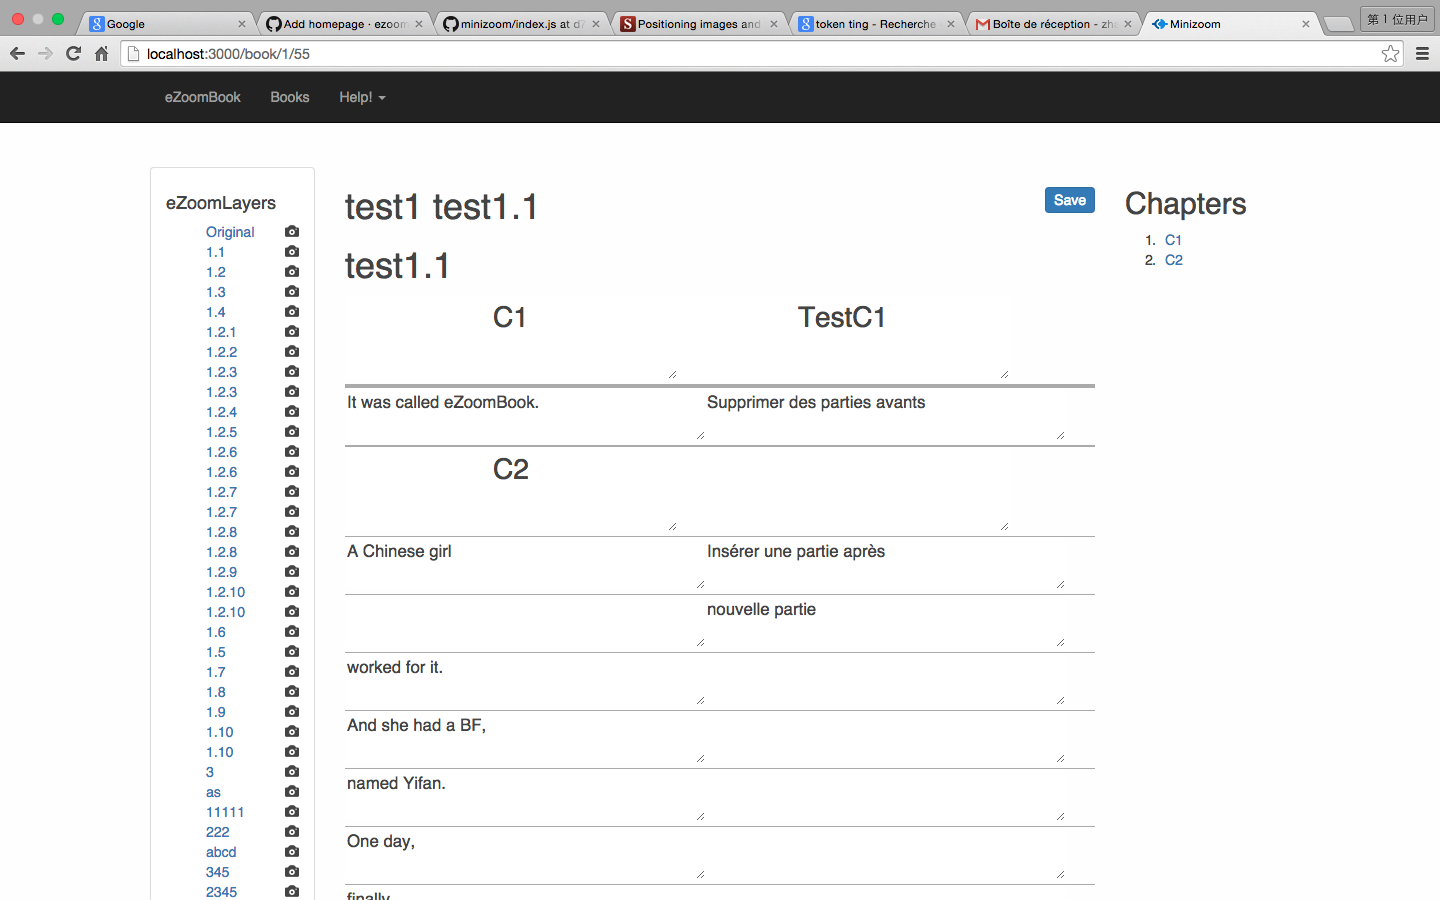
\includegraphics[width=\textwidth]{trans2}
\caption{Edition un nouveau layer}
\end{figure}

\subsection{Réalisation d'accès}

Pour réaliser un système d'accès fiable, j'ai choisi \textbf{Passport}, un module npm beaucoup utilisé qui permet d'indiquer des erreurs pour des utilisateurs.

\begin{figure}[H]
\centering
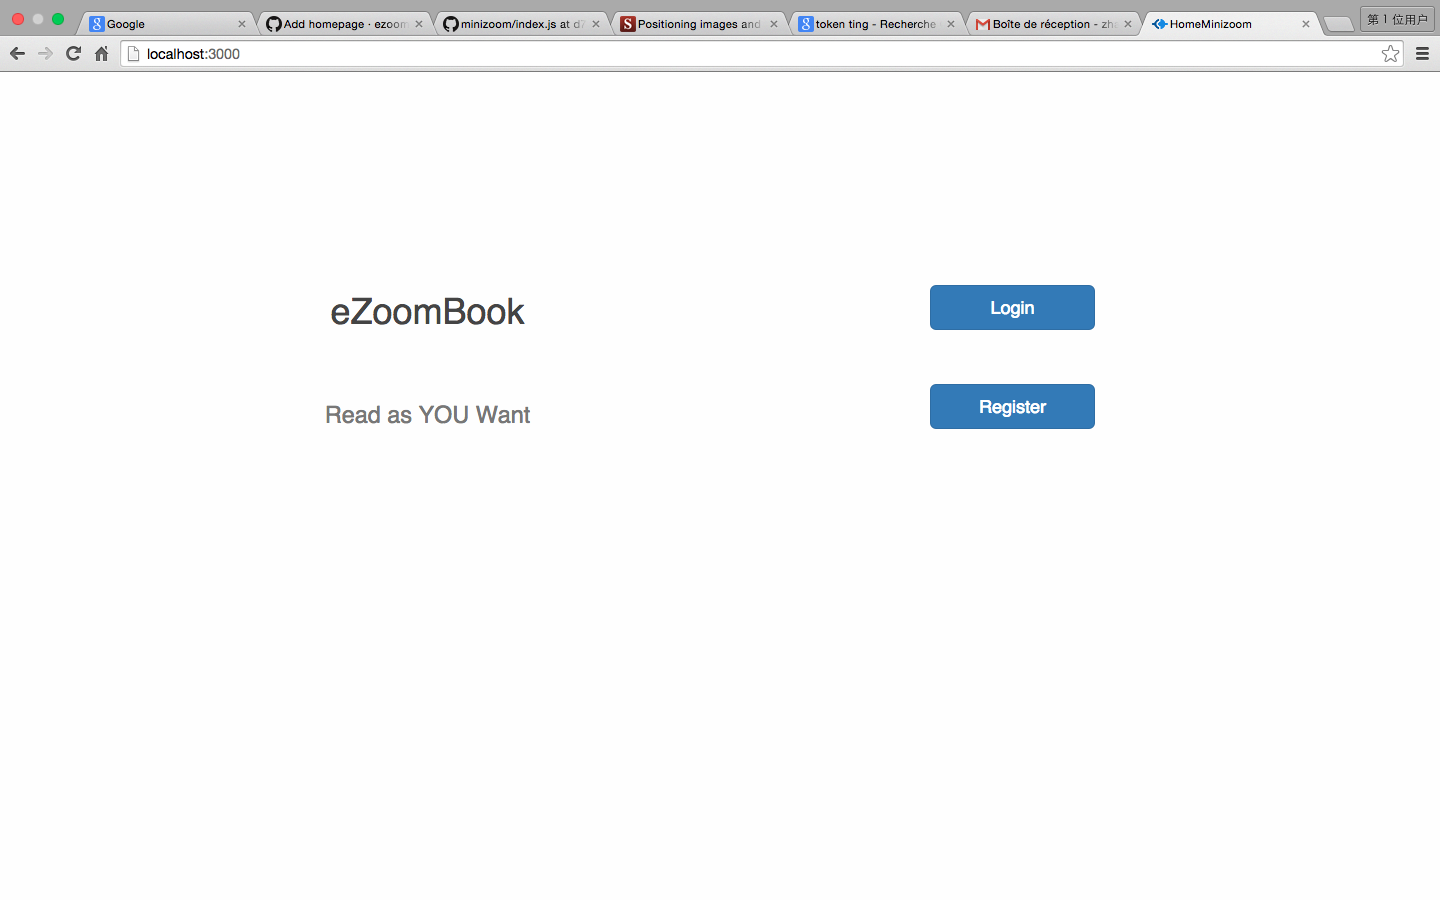
\includegraphics[width=\textwidth]{homepage}
\caption{Homepage}
\end{figure}

\begin{figure}[H]
\centering
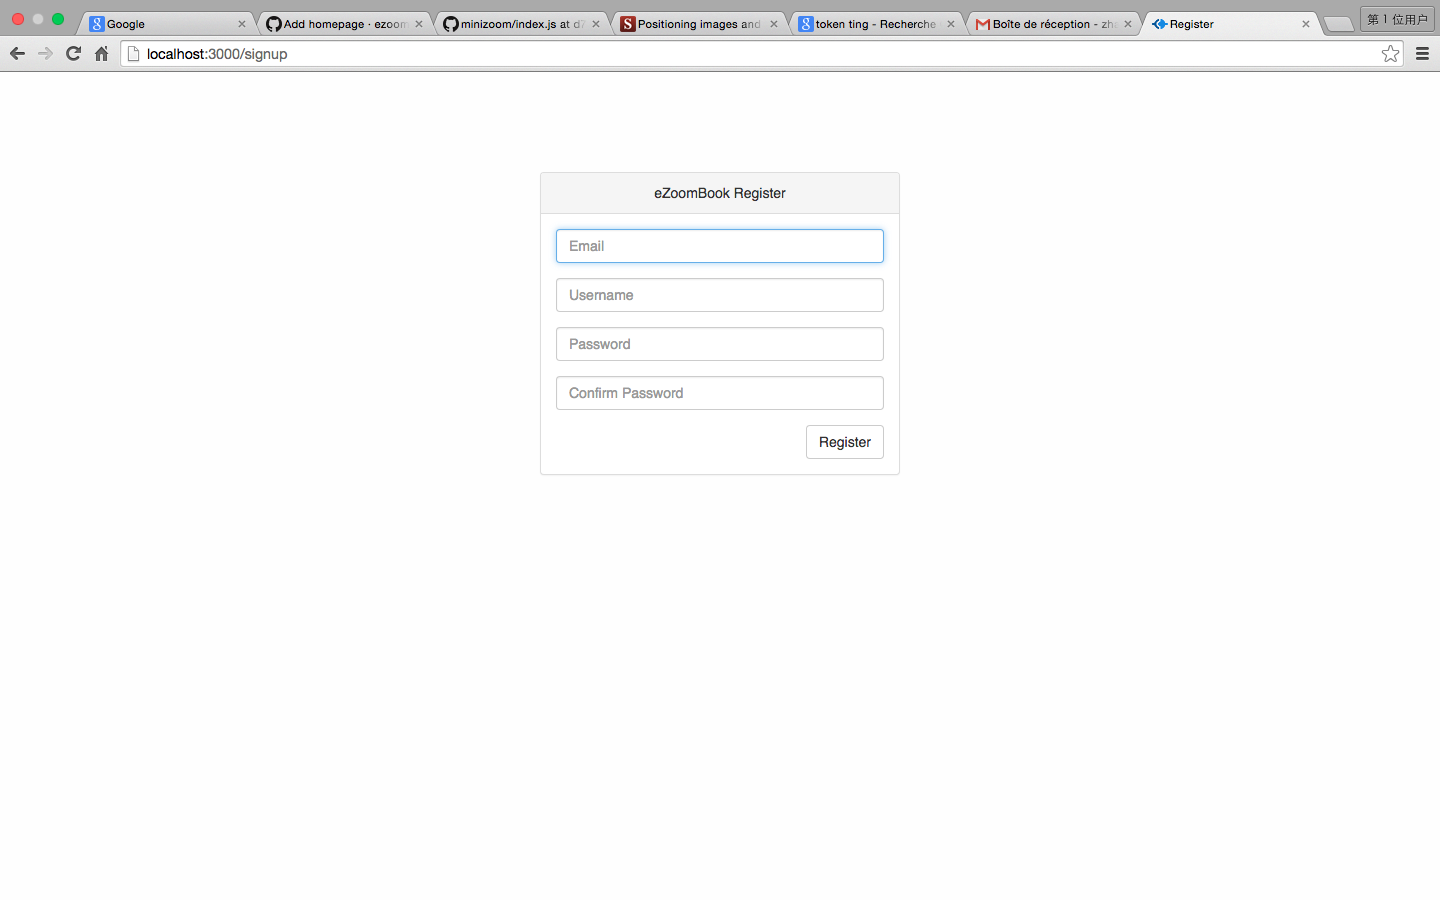
\includegraphics[width=\textwidth]{logup}
\caption{Logup}
\end{figure}

\begin{figure}[H]
\centering
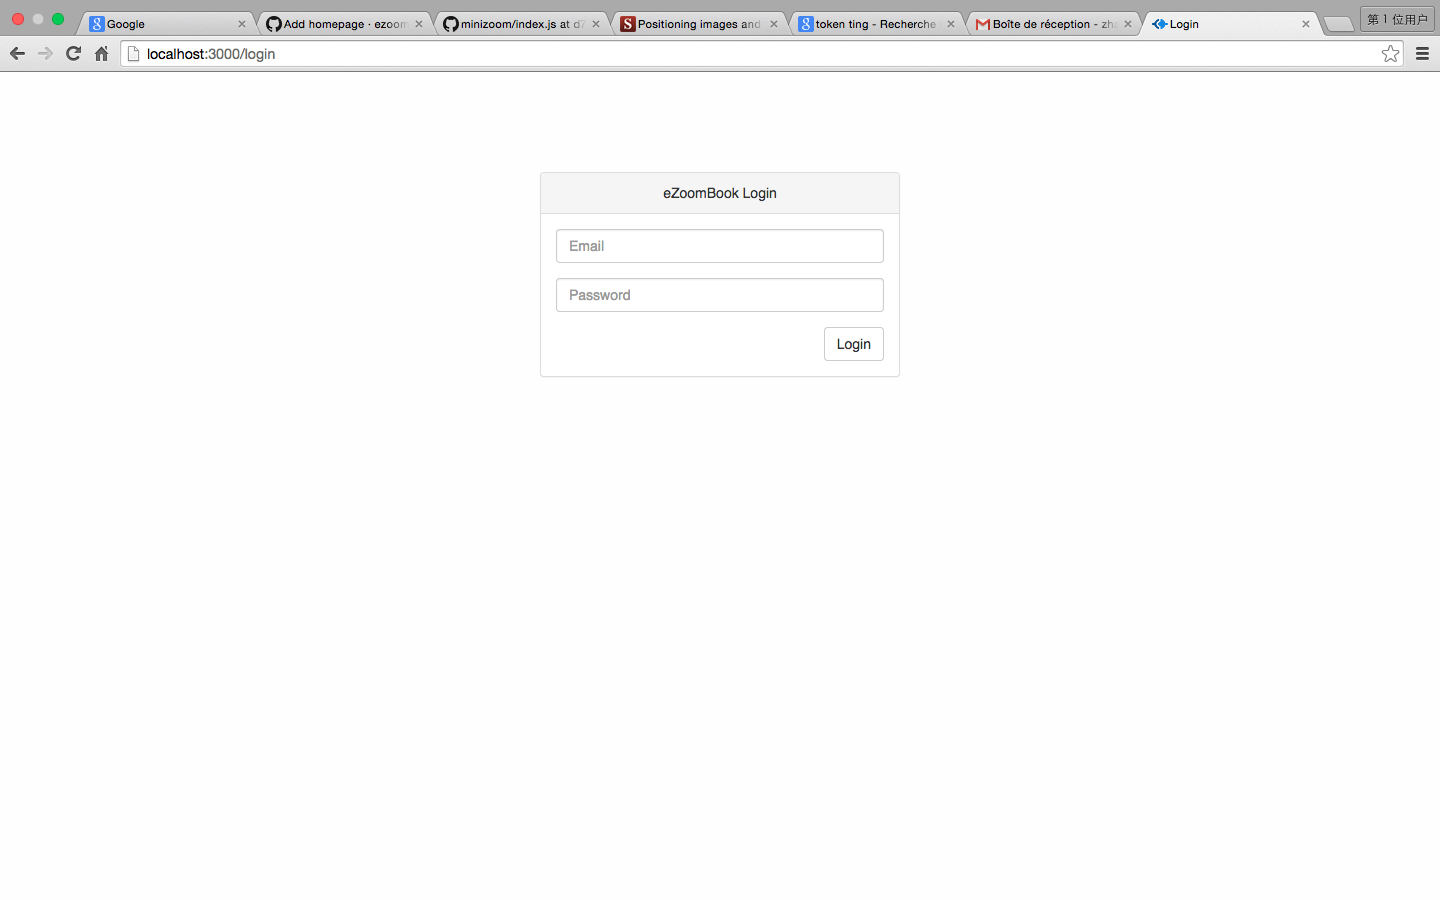
\includegraphics[width=\textwidth]{login}
\caption{Login}
\end{figure}

\subsection{Réalisation de la gestion d'utilisateurs}

\begin{figure}[H]
\centering
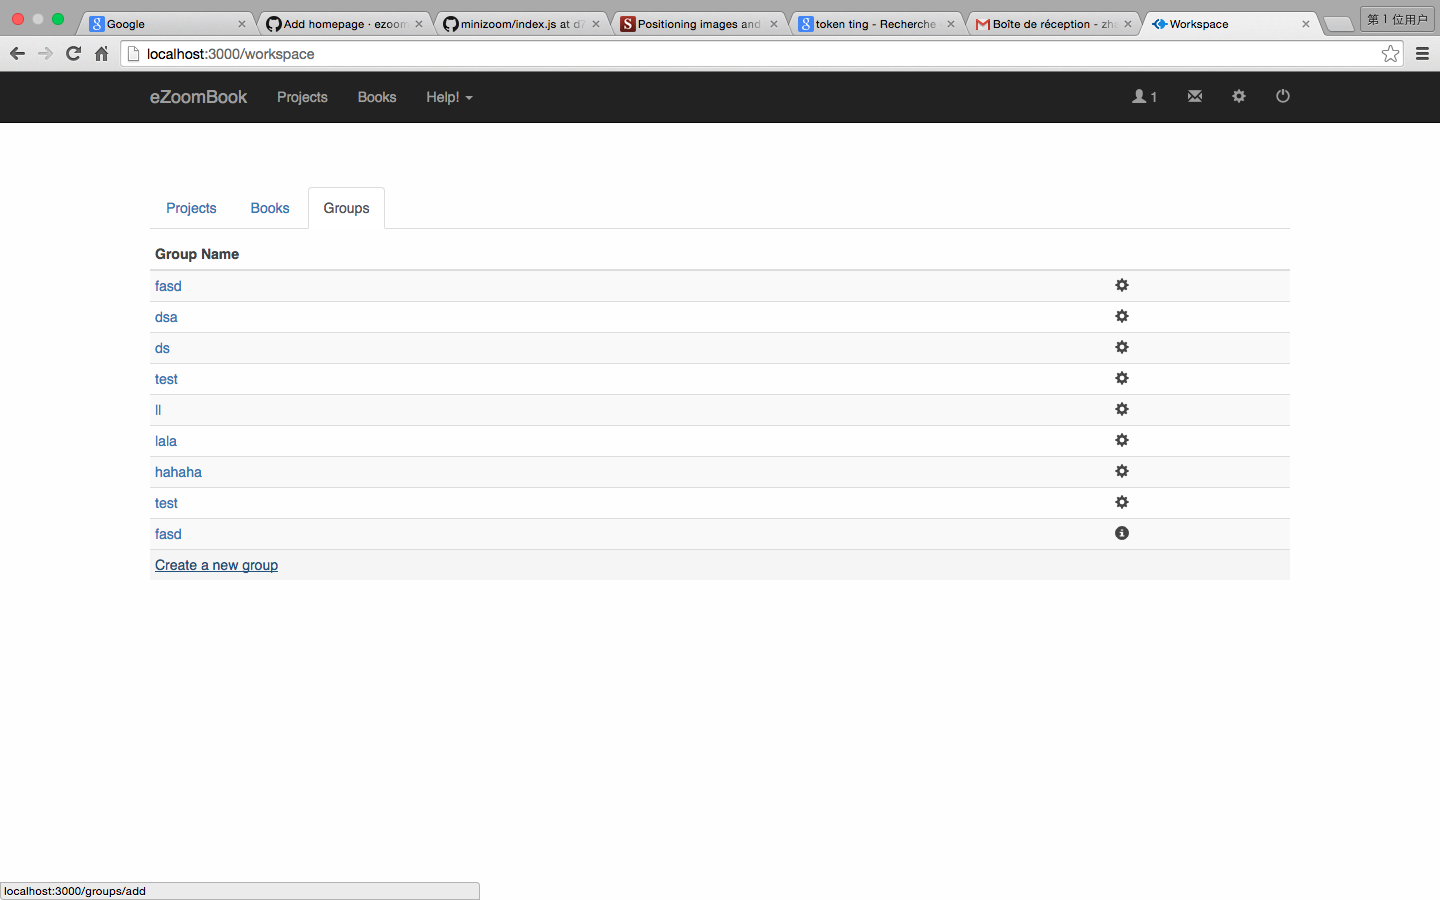
\includegraphics[width=\textwidth]{workspace}
\caption{Workspace}
\end{figure}

\begin{figure}[H]
\centering
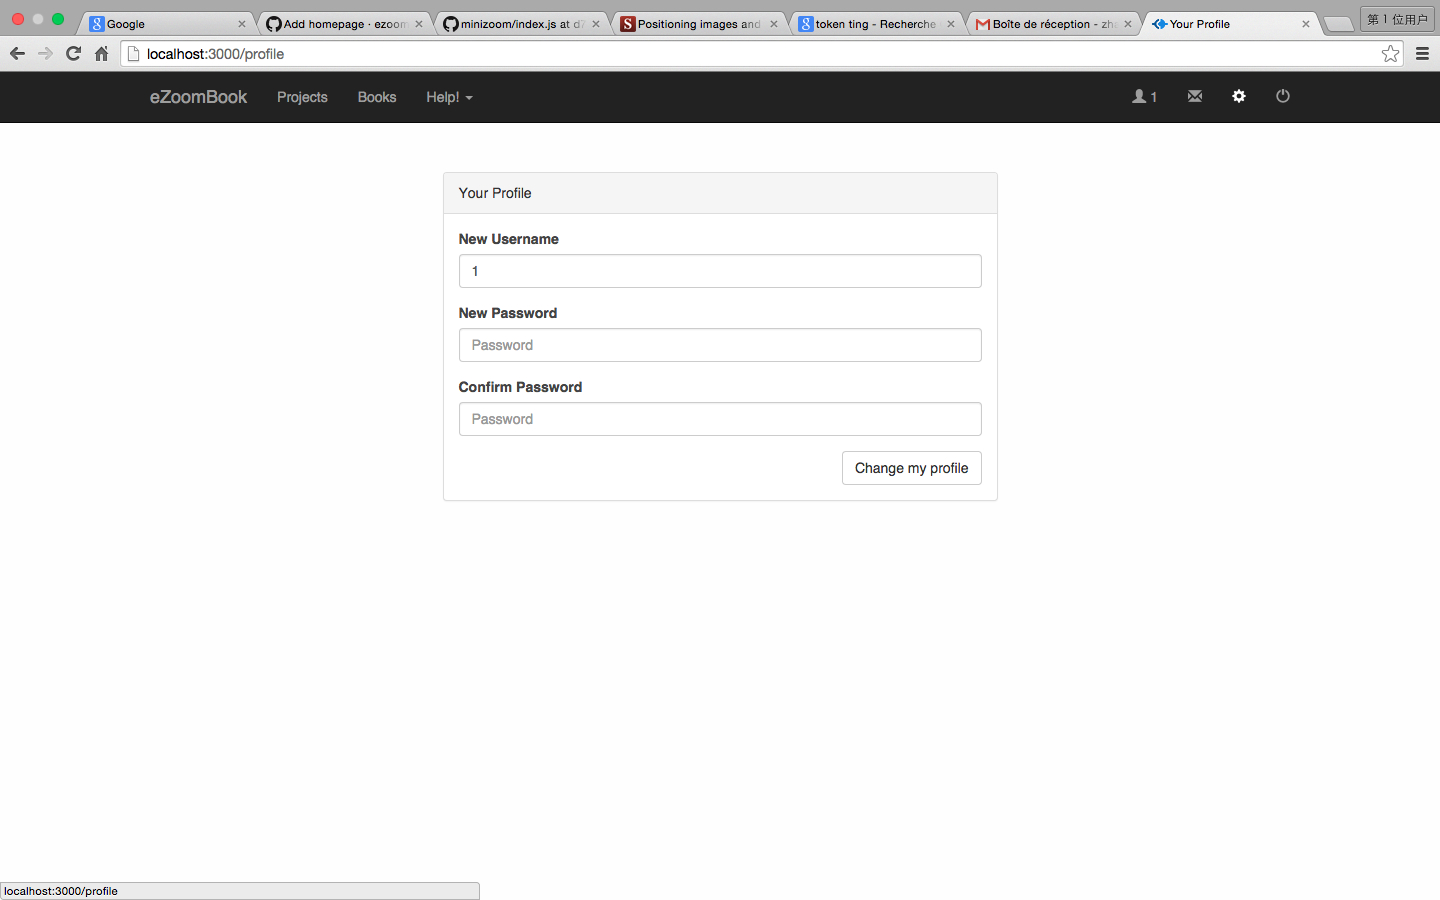
\includegraphics[width=\textwidth]{profile}
\caption{Changer des profiles}
\end{figure}

\subsection{Réalisation de la gestion de groupes}

\begin{figure}[H]
\centering
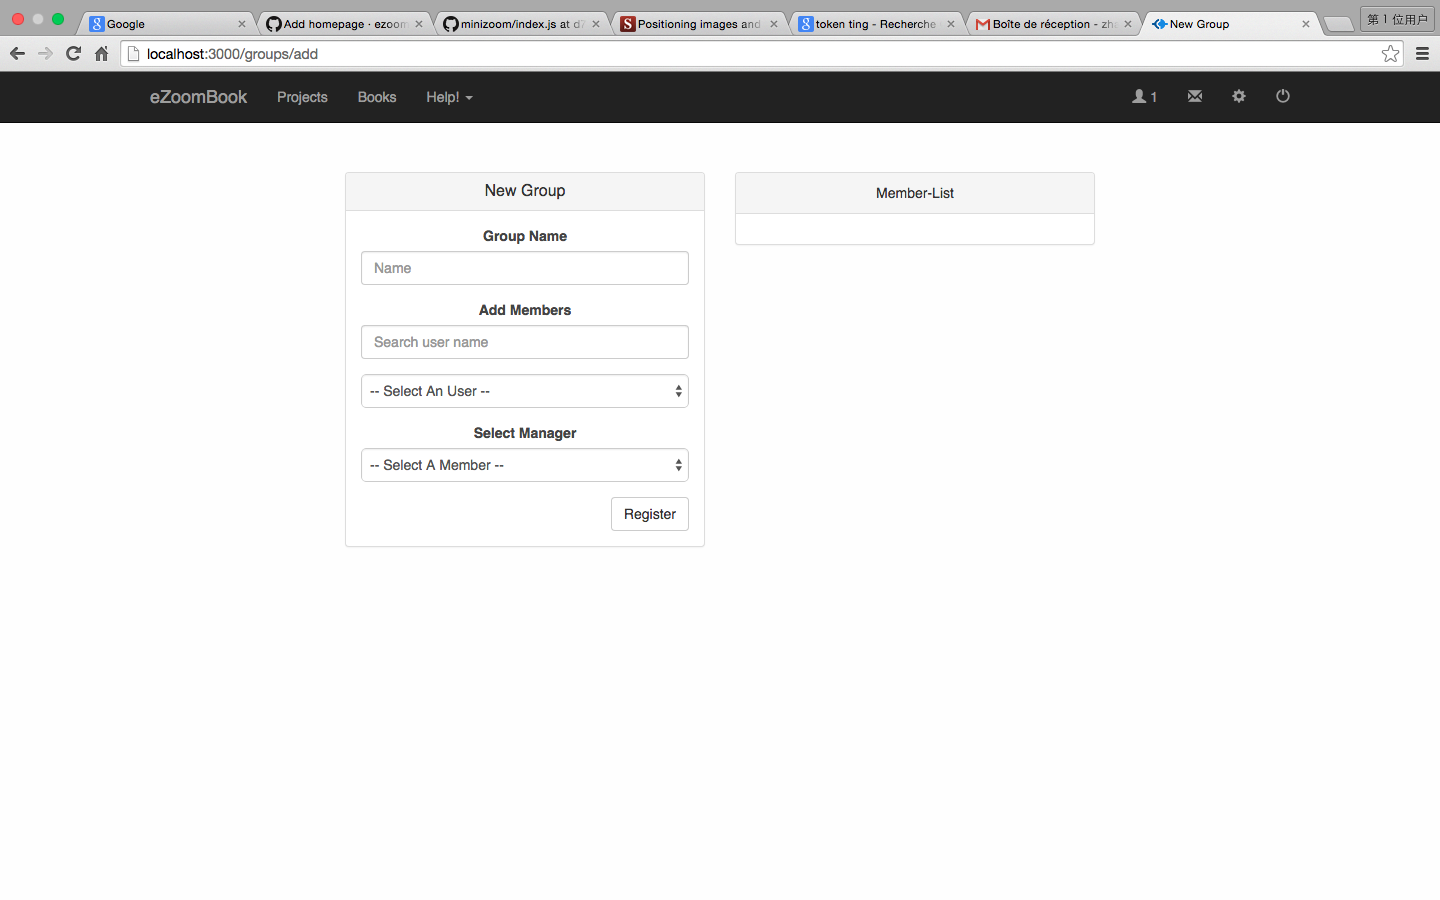
\includegraphics[width=\textwidth]{newgroup}
\caption{Créer un groupe}
\end{figure}

\begin{figure}[H]
\centering
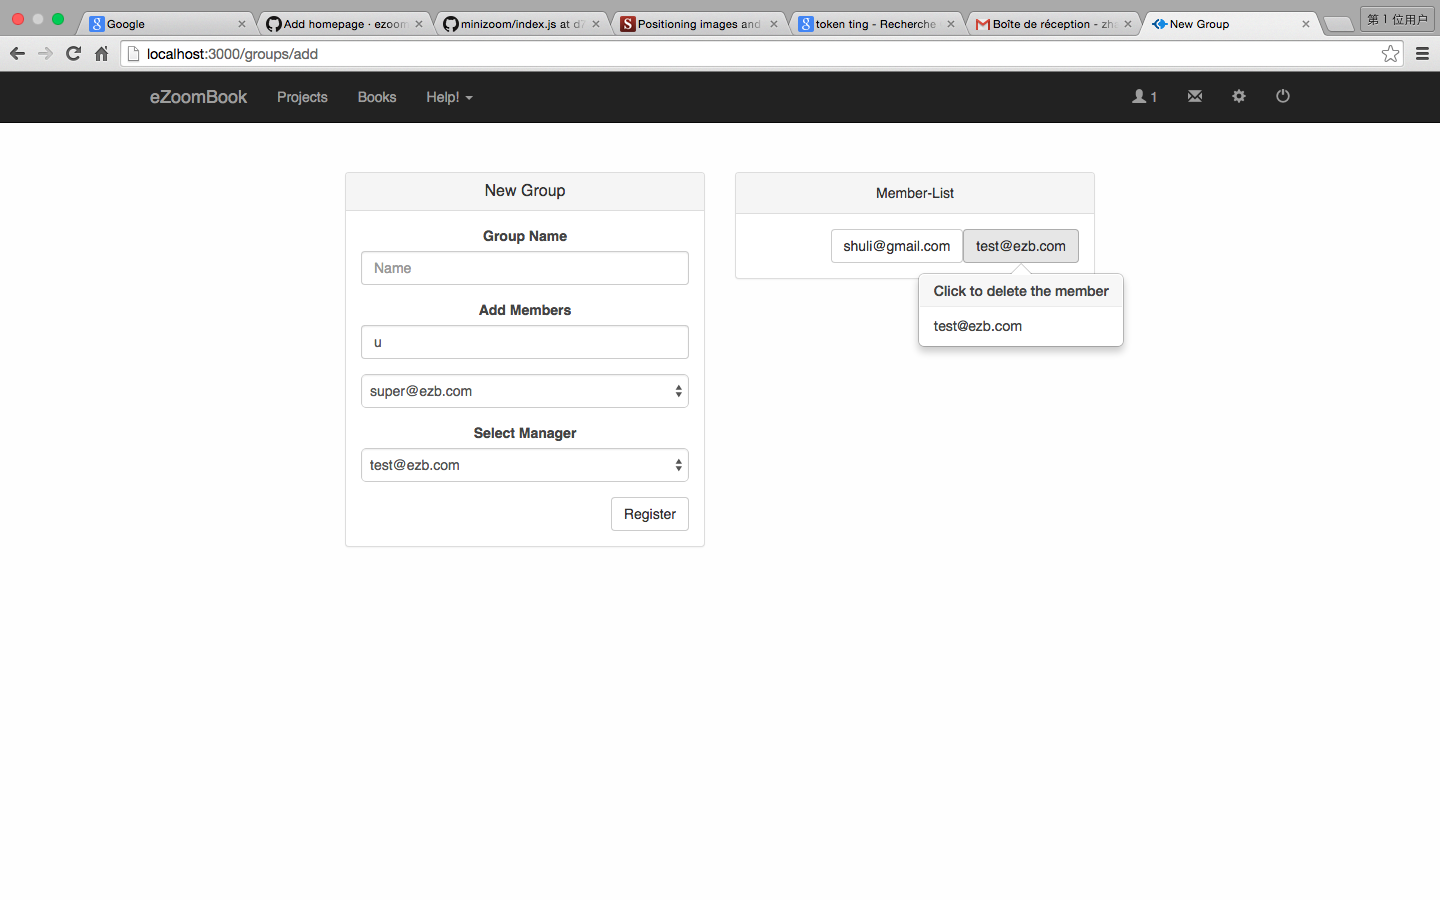
\includegraphics[width=\textwidth]{newgroup2}
\caption{Créer un groupe}
\end{figure}
